\section{Hierarchical Database Structure}

- Module ID
- Value Type
  - Scalar, Vector, Grid
- Location 
- Parameter
- Timeseries Type
  - sources - External, Simulated
  - category - Historical, forecast
- Time Step

\begin{figure}[htp]
    \centering
    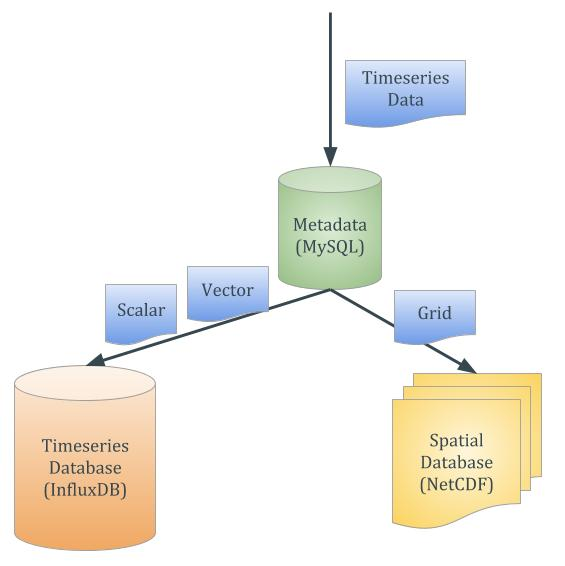
\includegraphics[width=1\textwidth]{method/microservice/hierarchical_database.jpg}
    \caption{Hierarchical Database}
    \label{fi:hierarchical_database}
\end{figure}

- MySQL
Relational Database Management System (RDBMS)

- InfluxDB \cite{influxdbInfluxDBDocumentation}
Open timeseries DB with MIT license
Support SQL-Like query language
Clustering available with a commercial version

- NetCDF \cite{unidataUnidataNetCDF}
Network Common Data Form
Self-describing, machine-independent data formats that support creation, access, and sharing of array-oriented scientific data
Support parallel file access

- MongoDB
  MongoDB is a general purpose, document-based, distributed database
  Supports query operations on geo-spatial data \cite{mongodbMongoDBManual}
  Clustering and Sharding available for scalability and reliability
  
- Redis \cite{redisRedisDocumentation}
  Redis is an open source (BSD licensed), in-memory data structure store, used as a database, cache.
  Clustering is available for scalability
  